\documentclass{article}
\usepackage[utf8]{inputenc}
\usepackage{graphicx}
\usepackage{amsmath }
\usepackage{amssymb}
\usepackage{subcaption}
\usepackage{float}
\usepackage{mathtools}
\setcounter{section}{0}


\usepackage{cleveref} %referencing figures, equations and tables
\crefformat{figure}{Figure.~#2#1#3}
\crefformat{equation}{Eq.~#2#1#3}
\crefformat{table}{Table.~#2#1#3}
\crefformat{appendix}{Appendix.~#2#1#3}
\crefformat{section}{Section.~#2#1#3}

\title{Propagation of a Shock Wave}
\author{Amir Baharvand }
\date{}

\begin{document}

\maketitle

The problem of propagation of a shock wave is given in \cite{Verruijt2010}. In the present solution, we discuss problems 7.3 to 7.4 of the same book.

\section{Displacement, Problem 7.3}
The displacement, $u$, due to propagation of a shock wave in a cavity in an infinite medium is

\begin{equation}
    u = \frac{pa^3}{4\mu r^2} \left \{ 1 - \left( \cos\theta - \frac{2r - a}{\alpha a}  \sin\theta \right) e^{-\dfrac{c_p\tau}{2da}} \right \} H(\tau)
    \label{eq:u}
\end{equation}

where

\begin{equation*}
    \begin{matrix}
    \alpha = \dfrac{1}{\sqrt{1-2\nu}} & , 
    \tau = t - \dfrac{r-a}{c_p} & , 
    d = \dfrac{1-\nu}{2-4\nu} & ,
    \theta = \dfrac{\alpha c_p\tau}{2da}
    \end{matrix}
\end{equation*}

\begin{equation}
    \begin{matrix}
    c_p = \sqrt{\dfrac{\lambda + 2\mu}{\rho}} & , 
    \lambda = \dfrac{E \nu}{(1 + \nu)(1 - 2\nu)} & ,
    \mu = \dfrac{E}{2(1 + \nu)}
    \end{matrix}
    \label{eq:consts}
\end{equation}

$p$ is the pressure, $a$ is the cavity radius, $r$ is the radial distance, $\nu$ is the Poisson's ratio, $t$ is time, $c_p$ is the wave propagation speed, $E$ is the Young's modulus, $\rho$ is density, $\lambda$ and $\mu$ are Lame's constants and $H$ is the Heaviside function. \\

The displacement on the boundary of the cavity ($r=a$) then reduces to

\begin{equation}
    u_0 = \frac{pa}{4\mu} \left \{ 1 - \left[ \cos \left(\dfrac{\alpha c_p t}{2da} \right) - \frac{1}{\alpha}  \sin \left(\dfrac{\alpha c_pt}{2da} \right) \right] e^{-\dfrac{c_p t}{2da}} \right \} H(t)
    \label{eq:u_0}
\end{equation}

\cref{fig:u_0_c_p} shows the displacement on the cavity boundary, $u_0$, for various Poisson's ratios. The time axis is normalized by $\dfrac{c_p}{a}$ where $c_p$ is determined from \cref{eq:consts}. $t$ can also be normalized by another parameter, $\dfrac{c_1}{a}$ where $c_1 = \sqrt{\dfrac{E}{\rho}}$ which is shown in \cref{fig:u_0_c_1}.

\begin{figure}[H]
    \centering
        \begin{subfigure}{0.49\textwidth}
            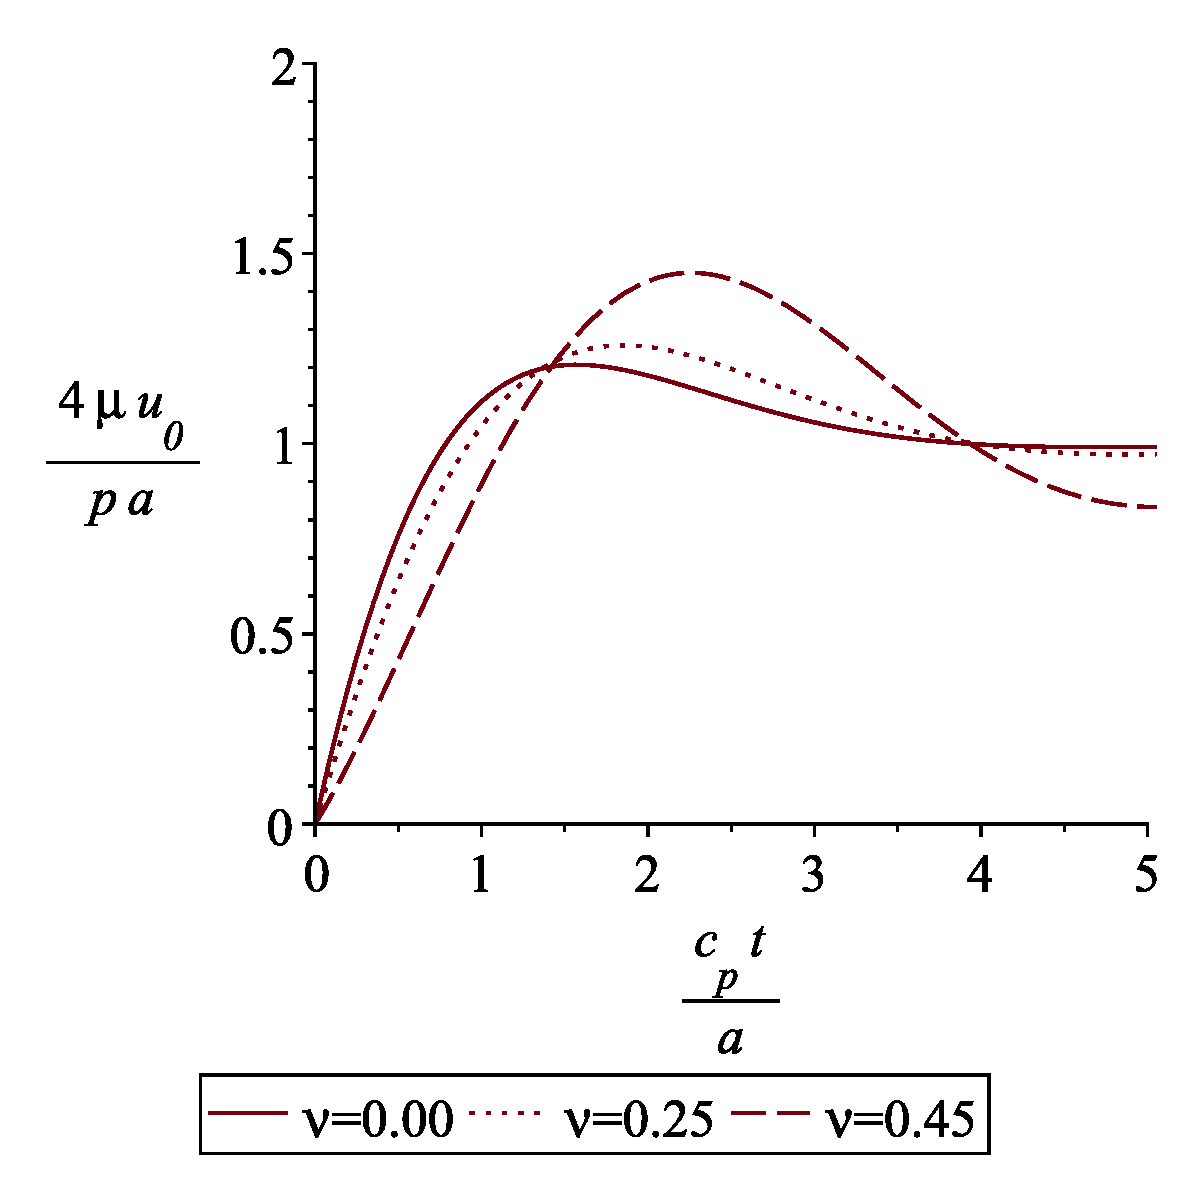
\includegraphics[width=1\linewidth]{figures/u_0_c_p.eps} 
            \caption{Normalized $t$ using $c_p$.}
            \label{fig:u_0_c_p}
        \end{subfigure}
        \begin{subfigure}{0.49\textwidth}
            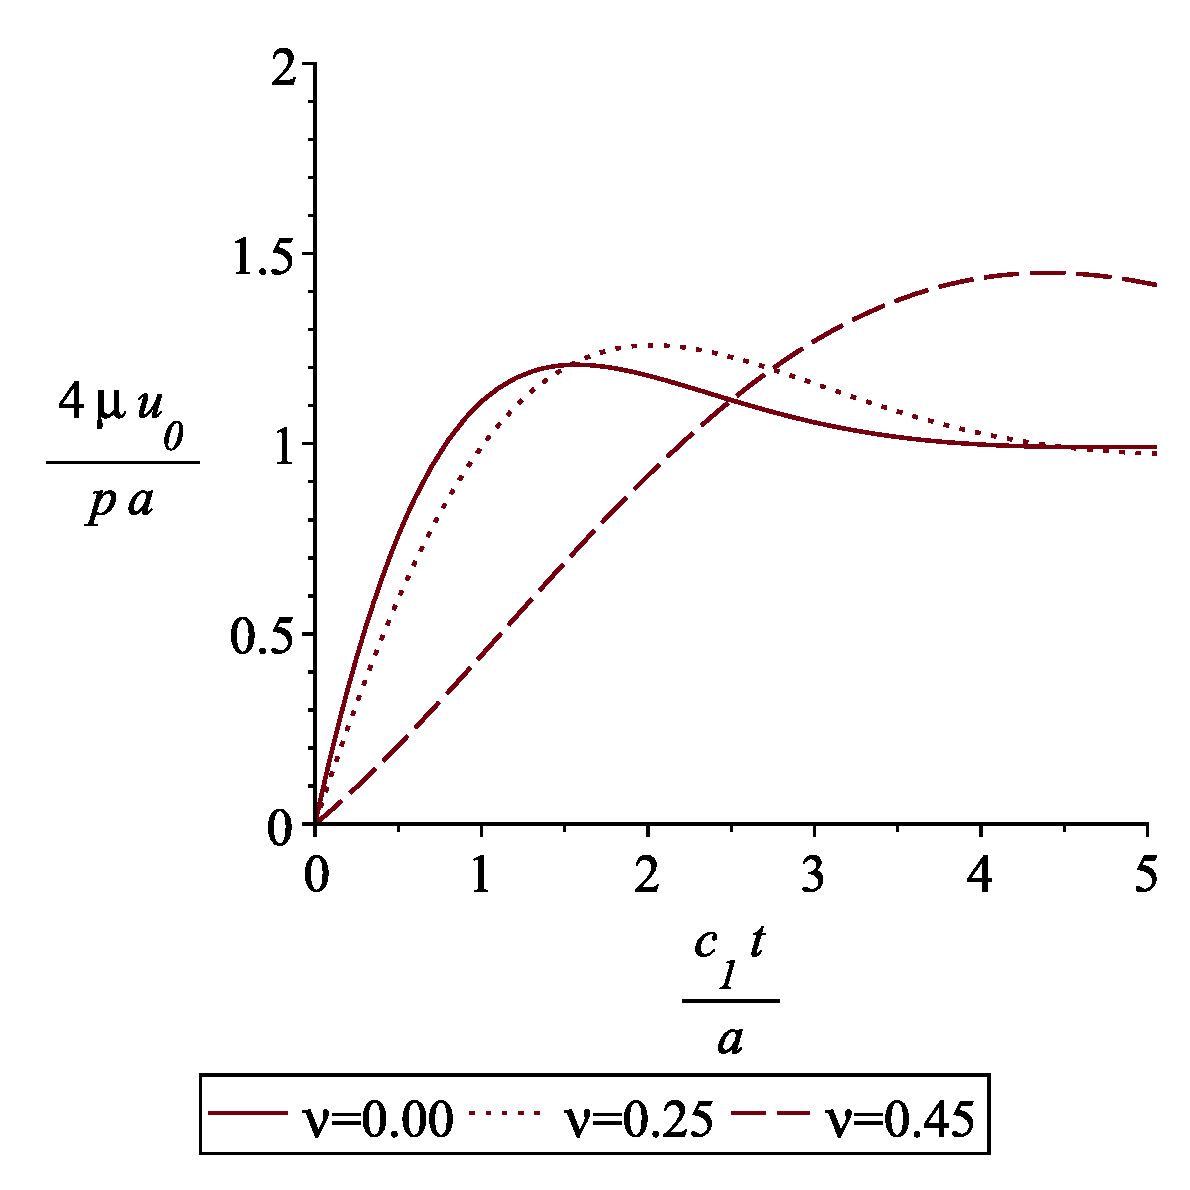
\includegraphics[width=1\linewidth]{figures/u_0_c_1.eps} 
            \caption{Normalized $t$ using $c_1$.}
            \label{fig:u_0_c_1}
        \end{subfigure}
    \caption{Normalized displacement on the cavity boundary ($r = a$).}
    \label{fig:u_0_c}
\end{figure}

One may notice that while $c_p$ is dependent on the Poisson's ratio (see \cref{eq:consts}), $c_1$ is not, which justifies different periods of plots for various $\nu$ in \cref{fig:u_0_c}. The period, $T$, of plots in \cref{fig:u_0_c} are summarized and compared in \cref{tab:period}. 

\begin{table}[H]
    \centering
    \begin{tabular}{c c c c c c} \hline
        $i$ & $\nu$ & $T_{c_p}$ & $\frac{T_{c_p,(i+1)}}{T_{c_p,i}}$ & $T_{c_1}$ & $\frac{T_{c_1,(i+1)}}{T_{c_1,i}}$ \\ \hline
        1 & 0 & 1.51 & - & 6.38 & - \\
        2 & 0.25 & 1.49 & 0.97 & 6.73 & 1.05 \\
        3 & 0.45 & 5.69 & 3.82 & 10.96 & 1.62 \\ \hline
    \end{tabular} 
    \caption{Periods of plots in \cref{fig:u_0_c} for $E$=1 and $\rho$=1.}
    \label{tab:period}
\end{table}

It is evident from the fourth and sixth columns of \cref{tab:period} that the periods of plots for different $\nu$ get closer if we normalize the time axis by $\dfrac{c_1}{a}$.

\section{Determination of the Stress Wave Traveling Time, Problem 7.4}
For this problem, the radial stress, $\sigma_r$, from \cref{eq:sigma_r} is plotted for a cavity of radius $a=1$m in soil with a wave propagation speed, $c_p=1000$m/s. 

\begin{equation}
    \sigma_r = -\frac{pa^3}{r^3} \left \{ 1 + \left( \frac{r^2 - a^2}{a^2}\cos\theta - \frac{1}{\alpha} \left(\frac{r-a}{a}\right)^2 \sin\theta \right) e^{-\dfrac{c_p\tau}{2da}} \right \} H(\tau)
    \label{eq:sigma_r}
\end{equation}

\begin{figure}[!]
    \centering
        \begin{subfigure}{0.64\textwidth}
            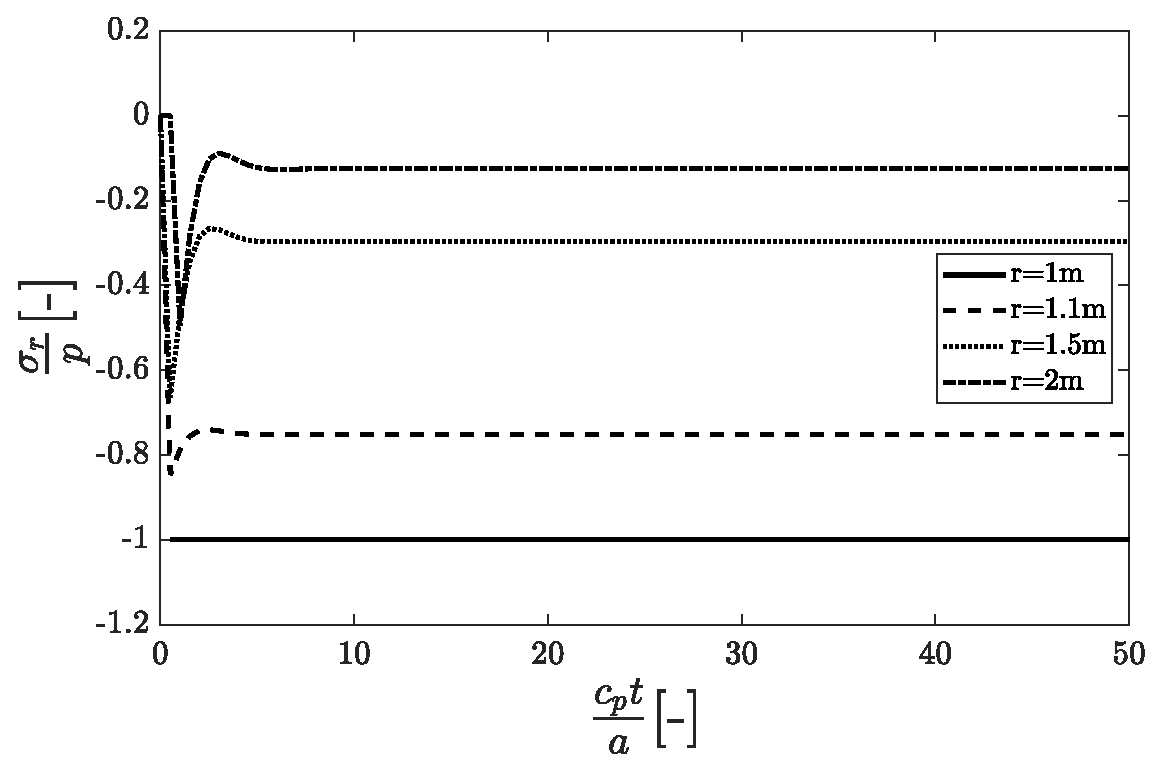
\includegraphics[width=1\linewidth]{figures/v0.eps} 
            \caption{$\nu = 0$}
            \label{fig:v0}
        \end{subfigure}
        
        \begin{subfigure}{0.64\textwidth}
            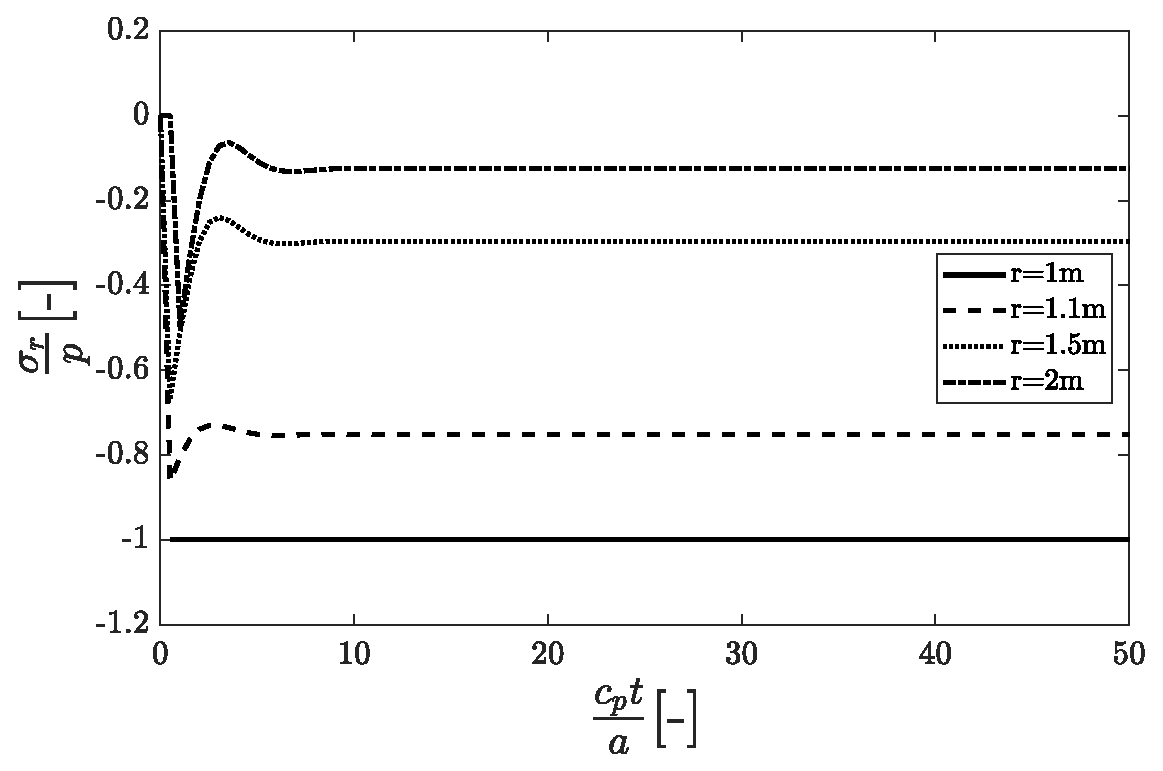
\includegraphics[width=1\linewidth]{figures/v0_25.eps} 
            \caption{$\nu = 0.25$}
            \label{fig:v0.25}
        \end{subfigure}
        
        \begin{subfigure}{0.64\textwidth}
            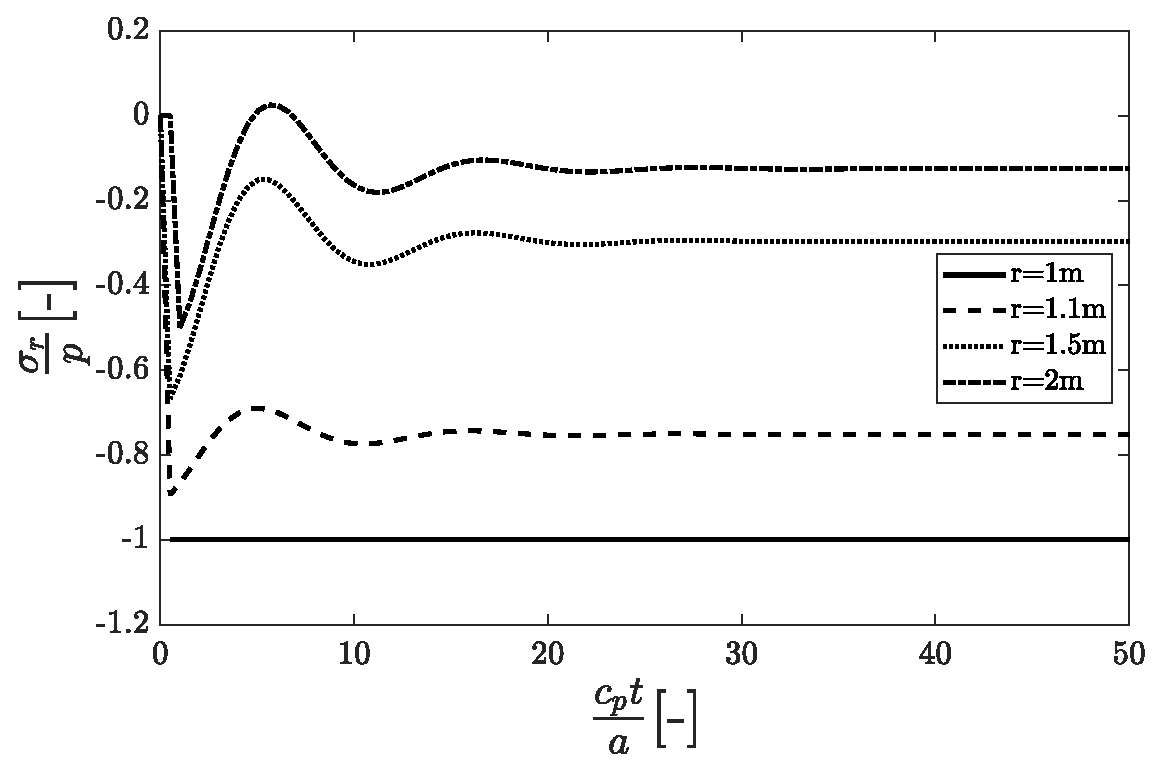
\includegraphics[width=1\linewidth]{figures/v0_45.eps} 
            \caption{$\nu = 0.45$}
            \label{fig:v0.45}
        \end{subfigure}
    \caption{Normalized radial stress for various values of $\nu$ at different distances, $r$, from the cavity.}
    \label{fig:7.4}
\end{figure}

$\alpha$, $\tau$, $d$ and $\theta$ can be found from \cref{eq:consts}. \cref{fig:7.4} provides a visualisation of $\sigma_r$ for three cases of $\nu$ at different distance, $r$, from the cavity. It is clearly visible that by increasing the Poisson's ratio, the required time to reach stability rises. For instance, for the case $\nu=0$, at $r = 2$m, $\sigma_r$ stabilizes at about $\dfrac{c_p t}{a}=$7.5, while the stability time for the same distance for $\nu=0.25$ and $\nu=0.45$ are 11 and 28, respectively. It is worth noting that the initial value of $\sigma_r$ is zero for the very first values of time and this mounts by increasing the radius. The reason behind this phenomenon is the wave propagation speed, as it takes some time for a point at distance to realize the generated stress wave. \\

By plotting the variation of Poisson's ratio for the range $0 \leq \nu \leq 0.45$ versus the stability time (\cref{fig:7.4_v_t_plot}) for $r=4a$, it is seen that the stability time monotonically rises by increasing $\nu$. It is worth mentioning that the relative error of less than 1\% for the value of radial stress is taken as the stability time criterion. \\

The stability time, in all the cases in \cref{fig:7.4}, decreases by moving further away from the cavity as a result of the damping coefficient (the exponential term in \cref{eq:sigma_r}). This falling behavior of stability time versus radius is plotted in \cref{fig:7.4_r_t_plot}. The first point in \cref{fig:7.4_r_t_plot} has the lowest value as in this case $r=a$; thus, the damping coefficient vanishes. The stability time criterion is chosen as the former case (the effect of Poisson's ratio on the stability time).\\

\begin{figure}[H]
    \centering
    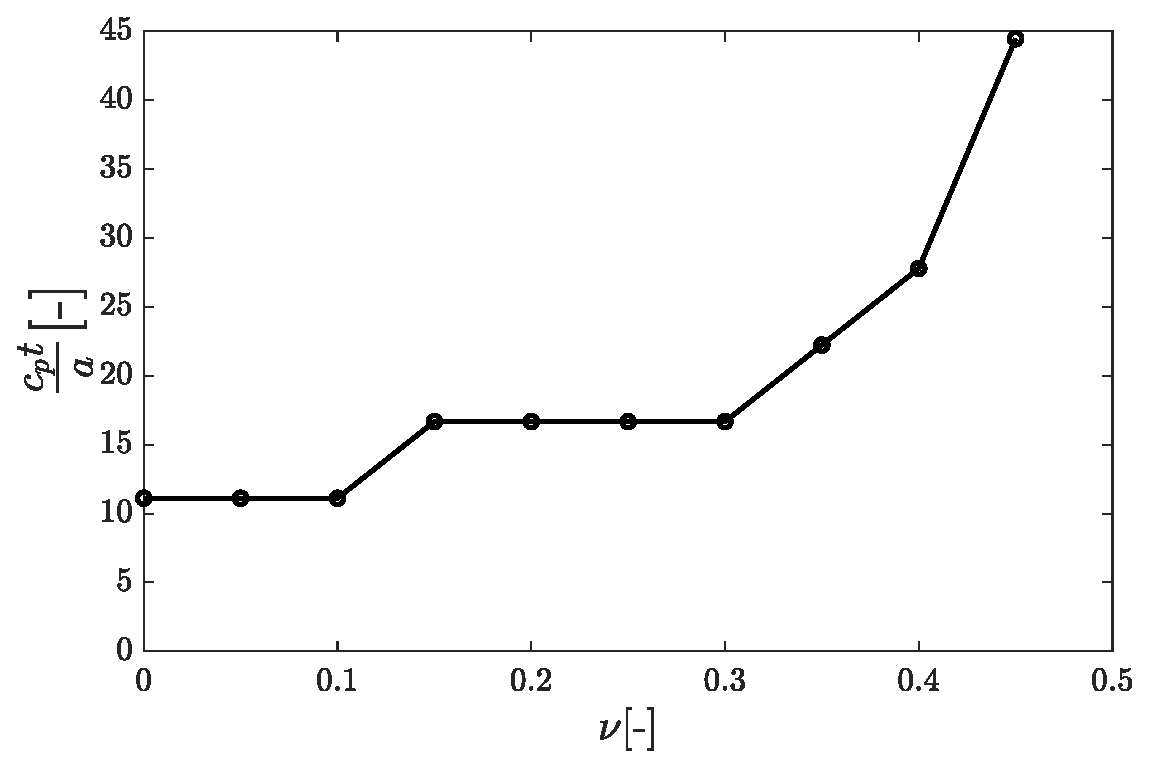
\includegraphics[width = 0.64\textwidth]{figures/v_t_plot.eps}
    \caption{The effect of Poisson's ration on stability time ($0 \leq \nu \leq 0.45$ at $r=4a$).}
    \label{fig:7.4_v_t_plot}
\end{figure}

\begin{figure}[H]
    \centering
    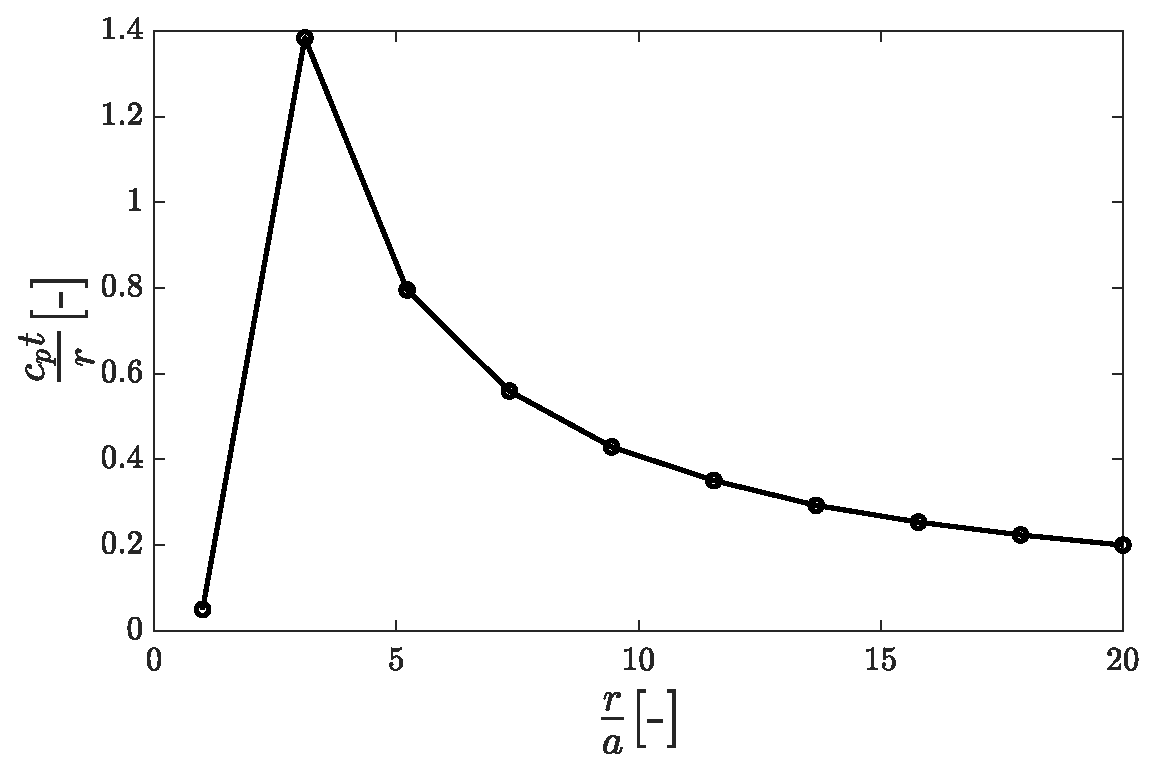
\includegraphics[width = 0.64\textwidth]{figures/r_t_plot.eps}
    \caption{The effect of distance from the cavity on stability time ($a \leq r \leq20a$ at $\nu=0.45$).}
    \label{fig:7.4_r_t_plot}
\end{figure}

\section{Determination of the Stress at Infinity, Problem 7.5}

Rewriting \cref{eq:sigma_r} and taking the limit when $\dfrac{r}{a} \to \infty$ results in zero stress which indeed coincides the radiation boundary condition ($\sigma_r = 0$ when $r \to  \infty$ for $t>0$). This vanishing point at infinite distance from the cavity for three cases of $\nu$ is also shown in \cref{fig:7.5}

\begin{equation*}
    \lim_{\textstyle\frac{r}{a} \to \infty} -\frac{pa^3}{r^3} \left \{ 1 + \left( \left[\left(\frac{r}{a}\right)^2 - 1 \right]\cos\theta - \frac{1}{\alpha} \left(\frac{r}{a}-1\right)^2 \sin\theta \right) e^{-\dfrac{c_p\tau}{2da}} \right \} H(\tau) = 0
\end{equation*}

\begin{figure}[H]
    \centering
    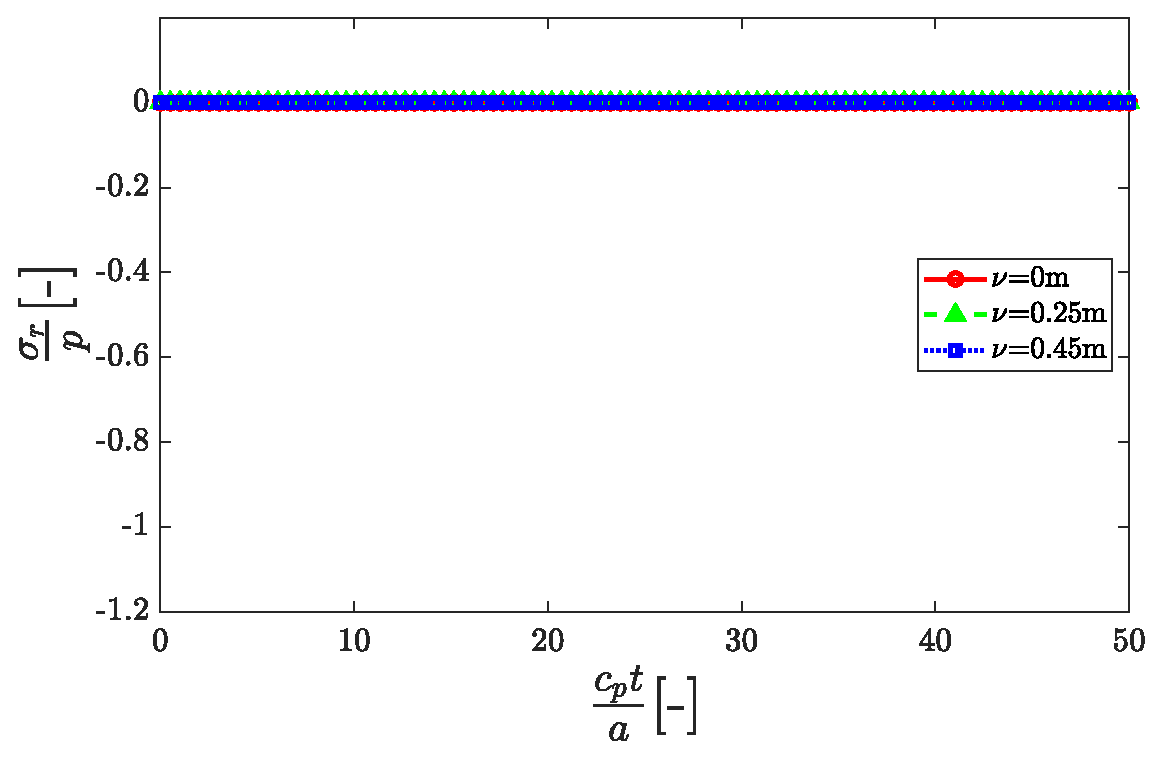
\includegraphics[width = 0.64\textwidth]{figures/large_r.eps}
    \caption{Normalized radial stress for various Poisson's ratios for $\dfrac{r}{a} \gg 1$.}
    \label{fig:7.5}
\end{figure}


\newpage
\bibliography{ref}
\bibliographystyle{ieeetr}

\end{document}